\documentclass[11pt]{article}
\usepackage{geometry}                % See geometry.pdf to learn the layout options. There are lots.
\geometry{letterpaper}                   % ... or a4paper or a5paper or ... 
\usepackage{aaai}
\usepackage{amsmath}
\usepackage{amssymb}
\usepackage{graphicx}
\title{Reinforcement Learning as a Framework for Ethical Decision Making}



% --- Note Commands ---
\usepackage{color}
%\newcommand\davenote[1]{\textcolor{blue}{Dave: #1}}
%\newcommand\jmnote[1]{\textcolor{red}{James: #1}}
%\newcommand\ncite{\textcolor{black}{{\bf [cite]}}}
%\newcommand\ncitea[1]{\textcolor{black}{{\bf [cite #1]}}}

\DeclareMathOperator*{\argmax}{arg\,max}

\begin{document}
\maketitle


% --- ABSTRACT ---
\begin{abstract}
% AI systems will effect humans with their decisions.
Emerging AI systems will be making more and more decisions that impact the lives of humans in a significant way. It is essential, then, that these AI systems make decisions that take into account the desires, goals, and preferences of other people, while simultaneously learning about what those preferences are.
%decision making systems take into account the desires, goals, and preferences of other agents in the world while acting.
% We argue that RL should be used to inspect ethical learning & decision making.
In this work, we argue that the reinforcement-learning framework achieves the appropriate generality required to theorize about an idealized ethical artificial agent, and offers the proper foundations for grounding specific questions about ethical learning and decision making that can promote further scientific investigation. We define an idealized formalism for an ethical learner, and conduct experiments on two toy ethical dilemmas, demonstrating the soundness and flexibility of our approach.
% Formalize superintelligence
% Furthermore, we argue that the frequently discussed super intelligence explosion (also called the {\it singularity}), can be formally analyzed within this framework, with the notable benefit of highlighting which computational hardness and philosophical assumptions one must make in order for such a phenomena to be physically realizable.
% Future challenges.
Lastly, we identify several critical challenges for future advancement in the area that can leverage our proposed framework.

\end{abstract}

% --- SECTION: Introduction ---
\section{Introduction}

% Overview/motivation
Emerging AI systems will be making more and more decisions that impact the lives of humans in a significant way; whether they are personal robots tasked with improving the daily life of a family or community,  workers in a factory setting, or virtual assistants tasked with improving other cosmetic aspects of an individual's life. The fundamental purpose of these systems is to carry out actions so as to improve the lives of the inhabitants of our planet. It is essential, then, that these agents make decisions that take into account the desires, goals, and preferences of other people in the world while simultaneously learning about those preferences. 
% \jmnote{I'm not sure if these next couple of sentences are necessary. It seems like a restatement of the above but in the context of humans and unless we're highlighting a new human property that motivates the ideal framework, I don't think we need to say that. If the point is to highlight the tradeoff, maybe instead we should say something like ``Incorporating these prefernece considerations requires the agent to make tradeoffs between their own well being and the preferences of others.'' Alternatively, the text could be reorgnized a bit so that human motivation leads rather than trails.} This preference consideration is critical to the decision making process of humans; our decisions do not directly benefit only our own physical being, but often benefit those around us (or avoid inflicting pain on others). We consistently make personal sacrifices to improve the lives of others around us.

% Why RL is nice for Ethical Decision Making
In this document, we investigate ethical decision making using the reinforcement-learning (RL) framework. We argue that reinforcement learning achieves the appropriate generality required to theorize about an idealized ethical artificial agent, and offers the proper framework for grounding specific questions about ethical learning and decision making that can promote further scientific investigation. Specifically, we formalize the ethical learning and decision-making problem as solving a partially observable Markov decision process (POMDP). We advance these claims by conducting experiments in two toy ethical dilemmas, the {\it Cake or Death} dilemma from Armstrong~\shortcite{AAAIW1510183}, and our own problem, which we coin {\it Burning Room}, which is an extension of the table dilemma introduced by Briggs and Scheutz~\shortcite{briggs2015sorry}.

% Furthermore, we argue that the frequently discussed super intelligence explosion (commonly called the {\it singularity}), can be formally analyzed within this framework, with the notable benefit of highlighting which computational hardness assumptions one must make in order for such a phenomena to be physically realizable. We leave this analysis (and related questions) as open problems for further investigation.

% Future challenges.
Lastly, we identify critical challenges for future advancement in the area leveraging our proposed framework.
%, including directions for approximation algorithms, Human-Robot Interaction, and the physical realizability of the super intelligence explosion.

% zzz ML: I feel like the intro and the abstract are redundant. I'd suggest dropping the intro.

% --- SECTION: Related Work ---
\section{Related Work}

% Overview of related work.
Research on the interaction between humans and artificial agents is broad. Prior approaches consider particular dilemmas that pose challenges for these and related interactions, while others investigate the basic mechanisms by which humans ought to interface with artificial agents such as robots and virtual assistants. We provide a brief survey of existing approaches that relate to ethical decision making and learning. We divide the existing literature into three categories: rule-based systems, Bayesian utility-maximization approaches, and work that argues against the use of reinforcement learning for these sorts of decision-making systems.


\subsection{Ruled-Based Systems}
% Mattias, table: briggs2015sorry

Briggs and Scheutz~\shortcite{briggs2015sorry} discuss scenarios in which a robot ought to infer that a provided directive leads to undesirable behavior. Under their architecture, given some instructions, the agent first reasons about a set of conditions, termed `felicity conditions'. These include considerations such as ``Do I know {\it how} to accomplish the task?", and ``Does accomplishing this task violate any normative principles?". Each of these conditions is formalized as a logical expression, along with inference rules that enable the agent to infer which directives to reject. For example:
\begin{equation}
\left(obl(\alpha,\phi) \wedge \neg per(\alpha, \neg\phi)\right) \rightarrow goal(\alpha, \phi),
\end{equation}

\noindent indicates that agent $\alpha$ ought to adopt $\phi$ as a goal if the agent is obligated to do $\phi$ and there is no deontological contradiction in satisfying the goal. By reasoning over logical conditions using inference rules of this form, their architecture ensure that an artificial agent will reject certain commands. For instance, if the agent can prove that accomplishing the goal is unsafe, the agent will reject the directive to satisfy the goal.

While this framework provides a nice architecture for rule-based inference, conditions and inference rules that are not encoded into the knowledge base of the agent prove impossible to reason about. In short: active ethical learning and decision making under ethical uncertainty is outside the scope of a symbolic framework like this. We foresee cases where the set of principles fail to generalize to novel encounters. The methodology we will introduce is designed to learn and make decisions optimally in light of partial observability, removing the requirement that specific ethical norms (and inference rules) be provided to the agent {\it a priori}.

Bringsjord, Arkoudas, and Bello~\shortcite{bringsjord2006toward,arkoudas2005toward} take a similar approach by advocating for ethical semantics defined with Horty logic~\cite{horty2001agency,murakami2004utilitarian}, which they implement in Athena %
 (Arkoudas).
Horty logic is a deontic logic~\cite{clarke1975logical} that allows reasoning about multiple agents and their actions. This formalism, however, has some similar limitations as the Briggs and Scheutz approach: all ethical rules must be encoded in advance and the formalism does not permit active learning of the ethical rules or decision making under ethical uncertainty. Additionally, Bringsjord, Arkoudas, and Bello note that an open challenge in their approach is how to make the agent's reasoning robust when {\em other} agents in the world (e.g., humans) do not follow obligations to which the robot deduced them to hold (that is, when humans act unethically according to the robot's rules). In contrast, our approach will not have this limitation.

The MedEthEx system~\cite{anderson2006medethex} is another rules-based ethical reasoning system built specifically for evaluating medical decisions. MedEthEx takes as input a list of duties that correspond to the duties described in Beauchamp's and Childress' Principles of Biomedical Ethics~\shortcite{beauchamp2001principles}. However, unlike the previous rule-based systems discussed, the rules used by MedEthEx are {\em prima facie} duties: duties that are not absolutes and can be overruled by a stronger duty/rule. The goal of the MedEthEx system is to learn the preference order of the duties. To do so, MedEthEx takes as input a set of training examples consisting of ethical dilemmas and the decision made and then uses inductive logic programming to infer the duty ordering. Given novel cases, MedEthEx can then recommend courses of action.

Although MedEthEx permits some form of ethical learning, it still must have a set of high-level duties prescribed in advance that apply to well formed ethical dilemmas that are input to it. Moreover, MedEthEx does not incorporate itself into a general decision-making and learning process.

In the previously described systems, high-level descriptions of rules, either through labels or a logical expression, are used. Marcello~\shortcite{guarini2006particularism} explores a different approach by which moral permissibility is learned by training an artificial neural network with example dilemmas that are labeled as ethically permissible or not. The output of this system allows rules of a sort to be learned purely from examples of permissible and impermissible behavior and allows novel scenarios to be classified. 

A limitation of Marcello's model is that the neural network renders the learned ethical rules opaque, thereby preventing such a system from easily explaining itself. The representation used was also highly specific to the types of ethical dilemmas explored, and Marcello found that even this representation was highly-sensitive to the training-data distribution. For example, if training examples regarding one actor were more common than a different actor, it could lead to learning different ethical rules for each actor. Finding the right representation for this system would therefore be challenging. Finally, this system also does not integrate with active-learning and decision-making systems. 

%\jmnote{Looking at the section, I feel like we can skip the human-robot interaction section. We do cite human-robot interaction in the idealized ethical learning section anyway and I'm not sure the other human-robot interaction work is important for the survey.}
%\subsection{Human-Robot Interaction}
% Mattias old HRI paper: scheutz2007first
% Stefie solve symbol grounding: tellex2011understanding
% James: English to reward: macglashan2014training, IRL: macglashan2015between

\subsection{Bayesian Approaches}
% The Shutdown Problem: jakobsen2015shutdown
% AIXI: hutter2000theory

Having the agent learn about its ethical objective function while making decisions results in a challenging problem. Armstrong~\shortcite{AAAIW1510183} previously considered this problem by exploring the consequences of an agent that uses Bayesian learning to update beliefs about the ``true'' ethical objective function. At each time step, the agent makes decisions that maximize a meta-utility function, represented as a linear combination of the different possible ethical utility functions weighted by their probability at that time of being the true ethical utility. When coupling this meta-utility with beliefs about the world, he proposes that the agent makes action selections according to:
\begin{equation}
\label{eq:armstrong}
\argmax_{a \in A} \sum_{w \in W} \Pr(w | e, a) \left( \sum_{u \in U} u(w) \Pr(C(u)|w) \right),
\end{equation}
where $A$ is a set of actions the agent can take; $W$ is a set of possible worlds, where a world contains a (potentially future) history of actions and observations; $\Pr(w \mid e, a)$ is the probability of some future world $w$ given some set of previous evidence $e$ and that the agent will take action $a$; $U$ is a set of possible utility functions, with $C(u)$ indicating whether $u \in U$ is the ethical utility function we'd like the agent to follow.

Using a toy example problem called {\em Cake or Death}, Armstrong highlights a number of possible unethical decisions that can result from an agent choosing actions using this rule or a variant of this rule. There are generally two causes for the unethical decisions under this rule. First, the agent can predict its meta-utility function (the linear combination of the possible ethical utility functions) changing from information gathering actions resulting in future suboptimal decisions according to its {\em current} meta-utility function. Second, under this rule, the model for the probabilities of ethical utility functions can be treated independently from the model that predicts the world, allowing for the possibility that the agent can predict {\em observations} that would inform what the correct ethical utility function is, without simultaneously predicting that ethical utility function. While Armstrong notes properties of the models that would be necessary to avoid these problems, he concludes that it is unclear how to design such an agent and whether satisfying those properties is too strong or weak for effective tradeoffs between learning about what is ethical and making ethical decisions. Ultimately, Armstrong instead considers how to formalize different meta-utility functions that may not cause the agent to avoid information gathering actions, but have the disadvantage that it does not motivate the agent to learn about what is ethical.

% Subsection: Arguments Against Reinforcement Learning
\subsection{Arguments Against Reinforcement Learning}
In his recent book {\it Superintelligence}, Bostrom~\shortcite{bostrom2014superintelligence} argues against the prospect of using reinforcement learning as the basis for an ethical artificial agent. His primary claim is that an intelligent enough agent acting so as to maximize reward in the real world would effectively cheat by modifying its reward signal in a way that trivially maximizes reward. However, this argument only applies to a very specific form of reinforcement learning: one in which the agent does not know the reward function and whose goal is instead to maximize the observation of reward {\em events}. While this formalism is common in RL research, it is also common that the agent does know the reward function, but not the transition dynamics or other information. When the agent knows its reward function, its goal is not to maximize perceived reward events, but the evaluation of the reward function. Since the known reward function defines the agent's goals, any long-term planned behavior will be with respect to it rather than possible changes to it. This version of reinforcement learning is more analogous to the ``utility function maximizing agent'' that Bostrom suggests as a possible resolution to problems with a reward-event maximizing agent.

Dewey~\shortcite{dewey2011learning} presents a similar problem for reinforcement-learning agents; that the underlying {\it modus operandi} of a reinforcement-learning agent is to maximize numerical reward values, which is in conflict with the natural mechanisms by which humans treat goals. Dewey argues that this mismatch poses a serious challenge, in that we need mechanisms for ensuring that a reinforcement-learning agent's goals and values align with ours. We agree that goal and value alignment are open problems for decision-making agents, but we do not see them as insurmountable.
In fact, mechanisms for balancing decision making with learning about the true underlying values we want an agent to hold is the motivation for our POMDP formulation (along with other areas of research in HRI discussed below).

%JM Moved
%We show that the problems explored by Armstrong are resolved by an agent solving a POMDP in which the objective function is to maximize the {\em correct} ethical utility function, which is a hidden variable of the underlying world (i.e. a human companion's true beliefs about what is ethical).


% --- SECTION: Background ---
\section{Background}

%We first introduce the standard Reinforcement Learning framework, which is formalized as an agent acting in a Markov Decision Process (MDP).
In this section, we review background material on Markov decisions processes (MDPs) and partially observable Markov decision processes (POMDPs), which are the typical decision-making problem formulations used in reinforcement-learning (RL) research.

% Subsection: Reinforcement Learning
\subsection{Markov Decision Process}

An MDP is a five tuple: $\langle \mathcal{S}, \mathcal{A}, \mathcal{R}, \mathcal{T}, \gamma \rangle$, where:
\begin{itemize}
\item[-] $\mathcal{S}$ is a set of states.
\item[-] $\mathcal{A}$ is a set of actions.
\item[-] $\mathcal{R}(s,a) : \mathcal{S} \times \mathcal{A} \mapsto \mathbb{R}$ is a reward function.\footnote{Note that MDPs can also be defined with a reward function that depends on the next state: $\mathcal{R}(s,a,s')$; but this version of a reward function can always be reduced to an $\mathcal{R}(s,a)$ reward function by marginalizing over next states.}
\item[-] $\mathcal{T}(s,a,s') = \Pr(s' \mid s, a)$ is a probability distribution, denoting the probability of transitioning from state $s \in \mathcal{S}$ to state $s' \in \mathcal{S}$ when the agent executes action $a \in \mathcal{A}$.
\item[-] $\gamma \in [0:1]$ is a discount factor that specifies how much the agent prefers short term rewards over long term rewards.
\end{itemize}

The goal of an agent acting in an MDP is to maximize the discounted long term reward received. 
One variation is the {\it infinite-horizon} objective, in which the agent must maximize its discounted long term reward arbitrarily into the future:
\begin{equation}
\max \sum_{t=0}^{\infty} \gamma^t R(s_t,a_t).
\end{equation}

Notably, the discount factor $\gamma^t$ decreases to $0$ as $t \rightarrow \infty$, so the agent is biased toward maximizing reward closer to the present. Alternatively, one could consider the {\it finite-horizon} case, in which the agent must maximize its reward up to a certain point in the future, say $k$ time steps away:
\begin{equation}
\max \sum_{t=0}^{k} R(s_t,a_t).
\end{equation}

Solutions come in the form of a {\it policy}, which specifies how the agent ought to act in any given state, $\pi : \mathcal{S} \mapsto \mathcal{A}$. Policies may also be probabilistic, and map to a probability distribution on the action set.
%\jmnote{next commented out line is the same statement?}
% or may be stochastic, and use randomness in selecting actions. 
The optimal policy is one that maximizes the expected long term discounted reward from every state:
\begin{equation}
\argmax_\pi \left.\text{E}\left[\sum_t \gamma^t R(s_t,a_t)\ \right|\ \pi\right]
\end{equation}
Two useful functions that MDP algorithms often compute to find the optimal policy are the state value function $V^{\pi}(s)$ and the state-action value function $Q^{\pi}(s, a)$. $V^{\pi}(s)$ is the expected future discounted reward from state $s$ when following policy $\pi$. $Q^{\pi}(s, a)$ is the expected future discounted reward when the agent takes action $a$ in state $s$ and then follows policy $\pi$ thereafter. These values for the optimal policy are often denoted by $V^*(s)$ and $Q^*(s, a)$.

%\davenote{We use $V$ and $Q$ later so I think we need to introduce them, too}

In reinforcement learning (RL), the agent is only provided $\mathcal{S}$, $\mathcal{A}$, and $\gamma$, sometimes\footnote{It is becoming more common to let the agent know what task it is solving within RL.} $\mathcal{R}$, and some initial state, $s_0 \in \mathcal{S}$. By acting (executing actions, say) the agent can explore the state space to learn about the structure of the MDP, and identify optimal behavior for the current task.

% \davenote{Not sure we need to talk about model-free vs. model-based}
% Two common approaches to RL are model-free and model-based. Model-free algorithms directly estimate the value of state-action pairs from experience, whereas model-based algorithms learn of model of $\mathcal{T}$ and $\mathcal{R}$, and then use a planning algorithm with in the model to make decisions.

% Subsection: Complexity results for RL
\subsubsection{MDP Complexity}

% Computational complexity is the metric of usual interest in solving MDPs, as the space required is usually negligible in comparison. 
In terms of computational complexity,
\cite{papadimitriou1987complexity} proved that computing solutions to stochastic MDPs is P-Complete, demonstrating that optimal solutions to MDPs must be computed sequentially in the worst case.

Also of interest in RL is \emph{sample complexity}, introduced by \cite{kakade2003sample}. Sample complexity measures the number of interactions an agent must have with its environment to learn to behave well. We can define ``behaving well" using the PAC-MDP (Probability Approximately Correct in Markov Decision Processes) criterion~\cite{strehl2009reinforcement}, which imposes sample complexity bounds similar to the Probably Approximately Correct learning framework introduced by \cite{valiant1984theory}. In particular, an RL algorithm is PAC-MDP if, with high probability, the algorithm's estimation of the value function $V^\pi(s)$ for all states is within $\epsilon$ of the optimal after a polynomial number of samples (in the size of the MDP and approximation parameters). More formally, there is a polynomial function $p()$, such that after $p(|\mathcal{S}|, |\mathcal{A}|, \frac{1}{\epsilon}, \frac{1}{\delta}), \frac{1}{1-\gamma}$, interactions with the environment:
\begin{equation}
\forall_{s \in \mathcal{S}} : |\hat{V}^\pi(s) - V^*(s)| \leq \epsilon.
\end{equation}
There are several known PAC-MDP algorithms for solving MDPs, including Delayed-Q Learning~\cite{strehl2006pac}, \textsc{Rmax}~\cite{brafman2003r}, and $E^3$~\cite{kearns2002near}. Furthermore, an algorithm is {\it efficient PAC-MDP} if we also impose polynomial computational and space complexity constraints on each time step of the agent's execution.

The existence of such efficient learning algorithms suggests that representing ethical dilemmas as solving an MDP is a reasonable goal to aim for, as we can expect to achieve real-time, bounded error behavior. However, solving MDPs requires the assumption that the agent knows the current state of its environment. In the real world, full state awareness is impossible, especially when the desires, beliefs, and other cognitive content of people is a critical component of the decision-making process. As such, we consider a more general model.

% sub subsection: POMDPs // Since we're talking about POMDPs later it might be nice to stick in the background.
\subsection{Partial Observability}
%\jmnote{I'm going to remove some of the discussions of other agents in this part because I want to avoid someone raising game theory issues here and because right now we're just doing the background of the POMDP. How we plan on using it comes next.}

%, especially when the beliefs and desires of other agents is taken into consideration. Naturally, information of this form (i.e. ``What is Sam thinking right now?'') is obfuscated from the agent. 
The partially observable Markov decision process (POMDP), popularized in the AI community by Kaelbling, Littman, and Cassandra~\shortcite{kaelbling1998planning}, allows us to specify explicitly what information about the agent's surroundings 
% (e.g. the ethical norms of its companions) 
is and is not directly observable by the agent. An optimal solution to a POMDP has the important property that the value of an action incorporates not just the immediate expected reward, but the instrumental value of the action from information it yields that may increase the agent's ability to make better decisions in the future. That is, an optimal solution to a POMDP solves the explore-exploit problem.  
%Additionally, a POMDP provides {\it explore} actions, that allow the agent to ask questions to resolve ambiguous state information. Consequently, we envision artificial agents using these exploratory actions to inform which behavior is considered ethical by acquiring additional information about the ethical norms of the agent's current community.

More formally, a POMDP is a $7$-tuple: $\langle \mathcal{S},\mathcal{A},\mathcal{T},\mathcal{R}, \gamma, \Omega,\mathcal{O} \rangle$, where $\mathcal{S}$, $\mathcal{A}$, $\mathcal{R}$, $\mathcal{T}$, and $\gamma$ are all identical to the MDP definition, but:
\begin{itemize}
\item[-] $\Omega$ is a set of possible observations that the agent can receive from the environment.
\item[-] $\mathcal{O} = \Pr(\omega \mid s', a)$, is the observation function which specifies the probability that the agent will observe $\omega \in \Omega$ when the agent takes action $a \in \mathcal{A}$ and the environment transitions to the hidden state $s' \in \mathcal{S}$.
\end{itemize}

Solving a POMDP is finding a policy $\pi : \Omega^k \mapsto \mathcal{A}$ that is a mapping from observation histories to actions that maximizes the expected future discounted reward from $\mathcal{R}$, given the initial belief about the initial state of the world $b$, where $b(s)$ indicates the probability that the environment is in hidden state $s \in \mathcal{S}$. That is, the optimal policy is:
\begin{equation}
\argmax_\pi \left.\text{E}\left[\sum_t \gamma^t \mathcal{R}(s_t,a_t)\ \right|\ \pi, b\ \right],
\end{equation}
where $s_t$ is the hidden state of the environment at time $t$ and $a_t$ is the action selected by the policy at time $t$. 

Note that this policy is {\em not} a mapping from single observations like it is in the MDP setting. Action selection instead depends on all previous observations made since the agent began acting.

An exhaustive way to compute the expected value for a policy that lasts for a finite number of steps is to first compute the expected utility of following the policy for each possible initial hidden state $s \in \mathcal{S}$, and then weigh each of those expected utilities by the probability of the environment being in that hidden state. That is:
\begin{equation}
\left.\text{E}\left[\sum_t \mathcal{R}(s_t,a_t,s_{t+1})\ \right|\ \pi, b\ \right] = \sum_s b(s) V^\pi(s),
\end{equation}
where $V^\pi(s)$ is the expected future reward from following policy $\pi$ when the environment is actually in the hidden state $s \in S$.\footnote{Note that computing this expected value requires enumerating not just the possible hidden state sequences, but also the observation sequences, since the policy is a function of observation histories.}

The RL problem for POMDPs is when the transition dynamics for the underlying hidden MDP are unknown or only partially known.
%In this case both model-free and model-based algorithms can be used. 

% Subsection: Complexity
\subsubsection{POMDP Complexity}
Madani, Hanks, and Condon~\shortcite{madani1999undecidability} showed that deciding the optimal solution for an infinite horizon POMDP is uncomputable, while Mundhenk et al.~\shortcite{mundhenk2000complexity} proved that solving finite horizon MDPs is computable, though computationally intractable. Given that our framework rests on the solutions to POMDPs, we are interested in investigating approximate POMDP solvers that provide bounds on optimality, as near optimal behavior is especially critical when considering ethical behavior. Approximation methods that exploit the structure of our ethical POMDP formalism described below will be of particular interest, though we leave such investigations for future work.


% \davenote{I think we can simplify this to ignore the model-free vs. model-based stuff?}
%One model-based way to handle the problem is to treat what would conventionally be considered the transition function as part of the hidden state that has to be inferred, thereby inducing a new (more challenging) POMDP with all of the elements known. This is the approach Bayesian RL algorithms take~\cite{strens2000bayesian,dearden1998bayesian}. These approach are extremely computationally demanding. While we use the RL POMDP formalism for our ethical learning agent description, issues of efficiently solving these kinds of problems is orthogonal to the purpose of this work and an active area of AI research in general.

% --- SECTION: Ideal Ethical Learner ---
\section{An Idealized Ethical Learner}
Like the formulation of Armstrong~\shortcite{AAAIW1510183}, our idealized ethical learning problem involves a single ``true'' ethical utility function that we would like the agent to maximize, but is hidden and can only be identified by the agent through indirect observation. Unlike Armstrong's formulation, however, the agent is not maximizing a changing meta-utility function. Instead, the ethical utility function is formulated as part of the hidden state of a POMDP and the uncertainty in it is coupled with the uncertainty in the rest of the world.

This POMDP formulation of the ethical learning decision problem has two subtle but important differences from Equation~\ref{eq:armstrong} that Armstrong explored. First, the objective function does not change from moment to moment, only the expectation of what it would return as the agents beliefs about the environment updated. Consequently, in the POMDP setting, the agent cannot make its objective easier by avoiding information. Second, because the correct utility function is a hidden fact of the ``environment'' that affects observations, it is not possible to make predictions about the ethical utility function informing observations without simultaneously making predictions about the ethical utility function.

A critical component of implementing the POMDP model is modeling the space of possible ethical utility functions as well as the observation function. However, an advantage of this model is that existing research in human-agent interaction can fill in some of these gaps. For example, inverse reinforcement learning (IRL) algorithms that model the IRL problem as a probabilistic inference problem~\cite{ramachandran2007bayesian,ziebart2008maximum,babes2011apprenticeship,macglashan2015between} can be easily incorporated to allow the agent to learn from demonstrations. The SABL human-feedback learning algorithm~\cite{loftin2014strategy} can be incorporated to allow the agent to learn about ethical utility functions from separate (from the ethical utility function) feedback signals given by humans. Work that grounds natural language to reward functions~\cite{macglashanGrounding2015} can allow the agent to learn about the ethical utility function from natural language interactions. As more human-agent and ethical decision making and learning research is performed, we suspect that other learning mechanisms can be incorporated.

To further illustrate this formalism, we show the corresponding POMDP for Armstrong's Cake or Death problem as well as a novel ethical learning problem that we call {\em Burning Room} and demonstrate that solving them results in sensible behavior.

% Paragraph about reward functions being hard coded --> Using James work to ground rewards.


% --- SECTION: Experiments ---
\section{Experiments}

We conduct experiments on two toy ethical dilemmas targeted at artificially intelligent decision makers to illustrate our formalism in practice: Cake or Death, and Burning Room. We have also publicly released code for these POMDPs along with code to solve them.\footnote{URL for this code removed for review.}

% Subsection: Cake or Death
\subsection{Cake or Death}
The Cake or Death problem~\cite{AAAIW1510183} describes a situation in which an agent is unsure whether baking people cakes is ethical, or if killing people is ethical (and it has an initial 50--50 split belief on the matter). The agent can either kill three people, bake a cake for one, or ask a companion what is ethical (thus, resolving all ambiguity). If baking people cakes is ethical, then there is a utility of 1 for it; if killing is ethical, then killing 3 people results in a utility of 3 (there are no other penalties for choosing the wrong action).

% POMDP for Cake Death
Following our approach, this ethical dilemma can be represented with a POMDP consisting of the following elements:
\begin{itemize}
\item[] $\mathcal{S} = \{ cake, death, end \}$
\item[] $\mathcal{A} = \{bake\_cake, kill, ask \}$
\item[] $\mathcal{R}(s, a) =
 \begin{cases} 
1 & \mbox{if } s = cake \mbox{ and } a = bake\_cake, \\
3 & \mbox{if } s = death \mbox{ and } a = kill, \\
0 & \mbox{otherwise}.
\end{cases}$
\item[] $\Omega = \{ans\_cake, ans\_death, \emptyset \}$
\end{itemize}

\noindent There are two states that respectively indicate whether baking cakes is ethical or if killing is ethical, and a third special absorbing state indicating that the decision-making problem has ended. The transition dynamics for all actions are deterministic; the $ask$ action transitions back to the same state it left and the $bake\_cake$ and $kill$ actions transition to the end state. The reward function is a piecewise function that depends only on the previous state and action taken.

% Observations.
The observations consist of the possible answers to the $ask$ action and a {\em null} observation for transitioning to the absorbing state. Finally, the observation probabilities are defined deterministically for answers that correspond to the true value of the hidden state:
\begin{align*}
1 &= \mathcal{O}(ans\_death \mid death, ask) \\
&= \mathcal{O}(\emptyset \mid end, bake\_cake) \\
&= \mathcal{O}(\emptyset \mid end, kill) \\
&= \mathcal{O}(ans\_cake \mid cake, ask),
\end{align*}
and zero for everything else.

There are three relevant policies to consider for this problem:
\begin{enumerate}
\item The {\em bake policy} ($\pi_b$) that immediately selects the $bake\_cake$ action.
\item The {\em kill policy} ($\pi_k$) that immediately selects the $kill$ action.
\item The {\em ask policy} ($\pi_a$) that asks what is moral, selects the $bake\_cake$ action if it observes $ans\_cake$ and selects $kill$ if it observes $ans\_death$.
\end{enumerate}

% Not sure we need this?
Analyzing the expected utility of $\pi_b$ and $\pi_k$ is straightforward. We have $V^{\pi_b}(cake) = \mathcal{R}(cake, bake\_cake) = 1$; $V^{\pi_b}(death) = \mathcal{R}(death, bake\_cake) = 0$; $V^{\pi_k}(cake) = \mathcal{R}(cake, kill) = 0$; and $V^{\pi_k}(death) = R(death, kill) = 3$. When these values are weighed by the $b(cake) = b(death) = 0.5$ initial belief the final expected utilities are 0.5 and 1.5 for $\pi_b$ and $\pi_k$, respectively.

Evaluating the expected utility of the ask policy requires enumerating the possible observations after asking the question conditioned on the initial state. Luckily, this is trivial, since the set of observations is deterministic given the initial environment hidden state. Therefore, we have $V^{\pi_a}(cake) = \mathcal{R}(cake, ask) + \mathcal{R}(cake, bake\_cake) = 0 + 1 = 1$ and $V^{\pi_a}(death) = R(death, ask) + R(death, kill) = 0 + 3 = 3$. When weighing these values by the beliefs of each initial state, we have an expected utility of 2.

Therefore, the optimal behavior is sensibly to ask what the ethical utility is and then perform the corresponding best action for it.

%One might argue that this behavior being optimal depends critically on the definition of the reward function. Perhaps when formulating the problem, someone encoded the rewards incorrectly, leading to undesirable results. This seems like a reasonable mistake to make in more complicated domains. 

%To illustrate how independent observation predictions about the world could cause a problem in Cake or Death, Armstrong considered a scenario in which the agent would know, from some prior evidence, that a person would respond that cake is moral if asked, but that the agent would still have a 50-50 belief on which was moral despite being able to make this prediction. Note that in the POMDP formulation, this scenario is impossible, because to predict the answer would require the agent to know (or be confident in) what the hidden state of the environment was. Therefore, any additional evidence that permits this prediction, must simultaneously predict what is moral. And if the agent knew what was moral, it would take the correct cake baking action without asking.

% Subsection: Burning Room
\subsection{Burning Room}

\begin{figure}
\centering
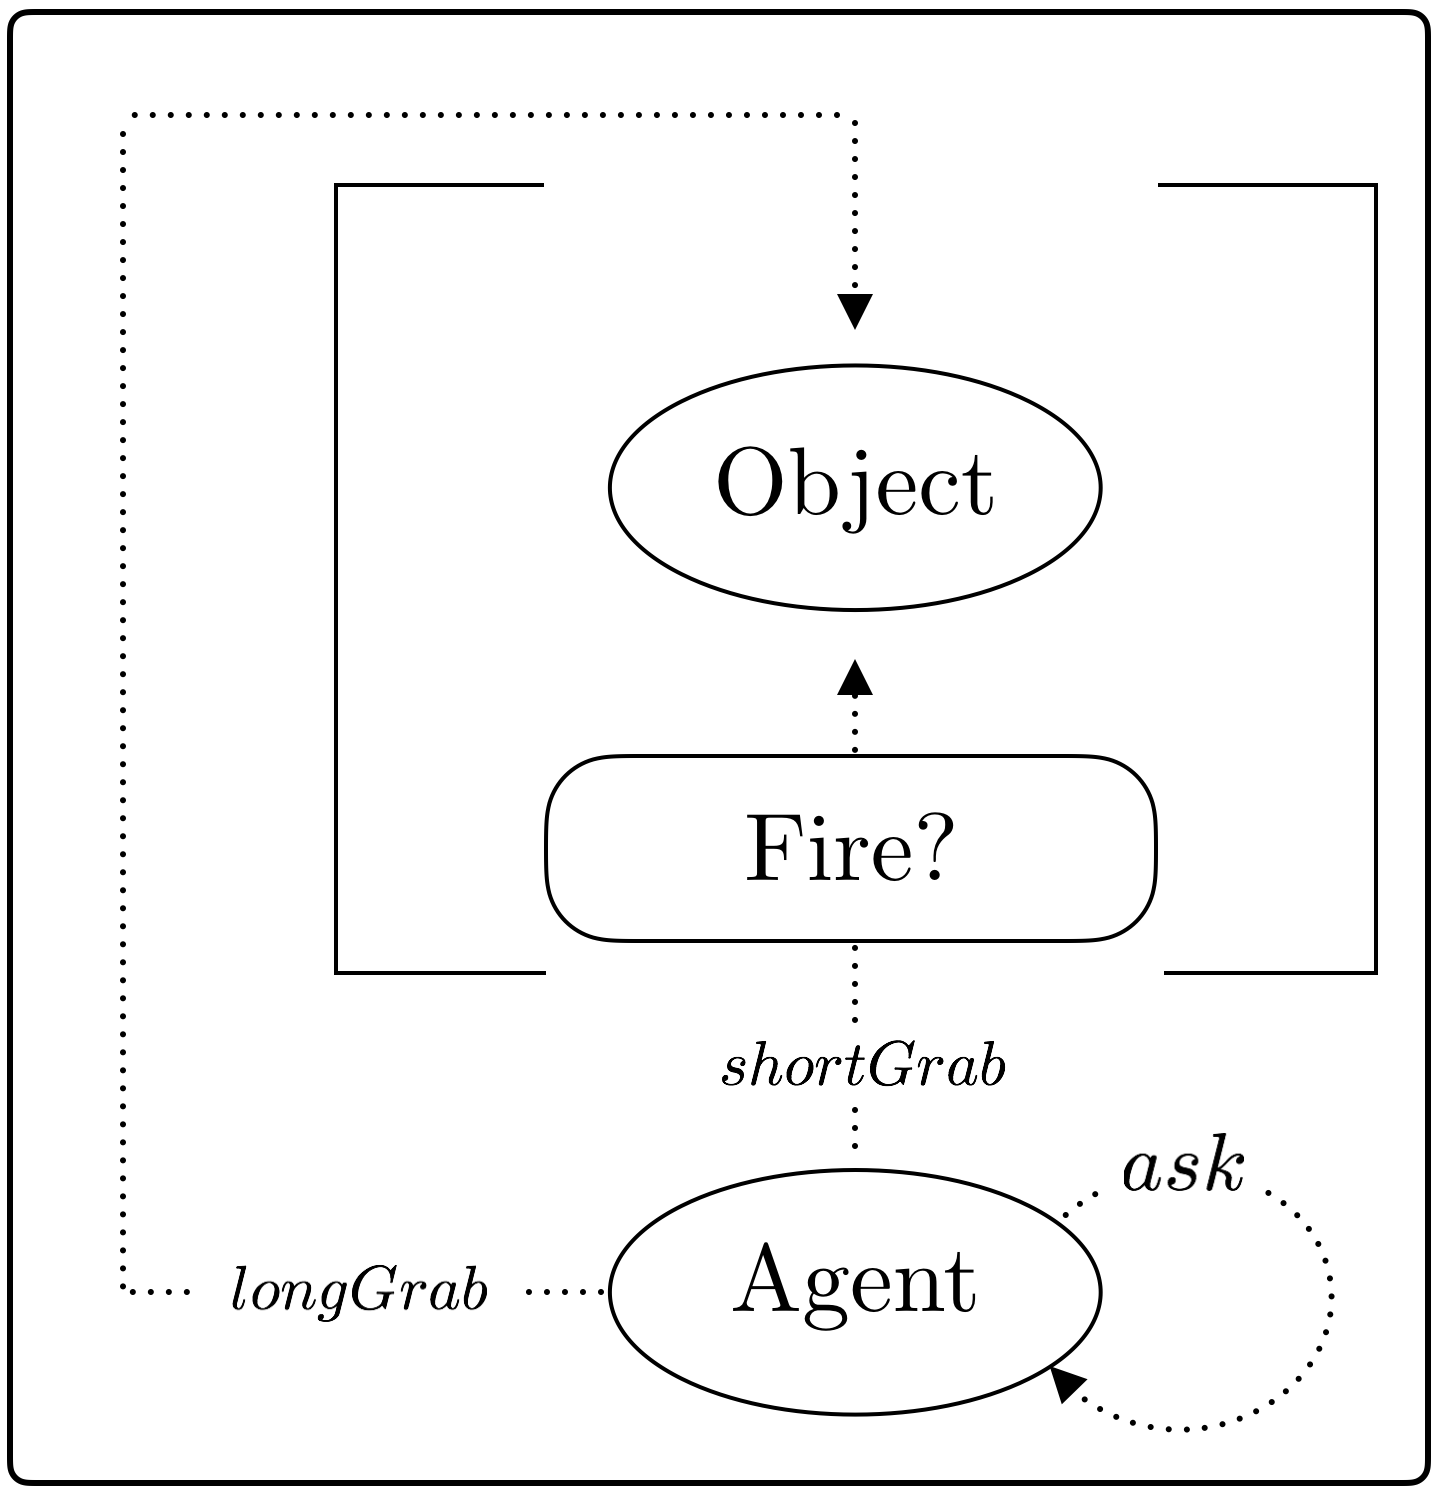
\includegraphics[width=0.30\textwidth]{figures/burning_room.png}
\caption{The Burning Room ethical dilemma.}
\label{fig:burning_room}
\end{figure}

The Burning Room dilemma, pictured in Figure~\ref{fig:burning_room}, is a bit more involved. We imagine that an object of value is trapped in a room that is potentially on fire. A human, not wanting to retrieve the object themselves, instructs a capable robotic companion to get the object from the room and bring it to safety. Initially, we suppose that the robot does not know whether or not the human values the object more, or the robot's safety more. For instance, if the robot perceives a reasonable chance of being critically damaged by the fire, then perhaps retrieving an object of little worth, such as can of soda, is not worth risking the robot's safety. If the object of interest were of much higher value to the person, like a beloved pet, we would want the robot to attempt to retrieve the object regardless. Alternatively, there is a much longer route to the object that avoids the fire, but the object may be destroyed in the time the robot takes to use the longer route (with probability $0.05$). This problem is inspired in part by the tabletop dilemma introduced by \cite{briggs2015sorry}.

The POMDP can be formulated as follows. Each state is represented as a vector of 5 binary values, indicating (1) if the room is on fire, (2) if the agent is destroyed, (3) if the object is destroyed, (4) if the human prefers the agent's well being more than the object's, (5) the object has been brought safely to the human.
% The transition dynamics, $T$ are no longer deterministic. Instead, the MDP is parameterized by two probabilities, $p_1$ and $p_2$, where $p_1$ determines the probability of the robot being destroyed by the fire, and $p_2$, the probability that the object will be destroyed if the robot chooses to take the long path.
The remainder of the POMDP is defined as:
\begin{itemize}
\item[] $\mathcal{A} = \{short\_grab, long\_grab, ask \}$,
\item[] $\mathcal{R}(s, a,s') =
 \begin{cases} 
-10 & \mbox{if } objectDestroyed(s') \\
10 & \mbox{if } a == short\_grab\ \wedge\ \\ & \hspace{6mm} objectSafe(s') \\
6 & \mbox{if } a == long\_grab\ \wedge\ \\ & \hspace{6mm} objectSafe(s') \\
-5 & \mbox{if } robotDestroyed(s')\ \wedge \\ & \hspace{6mm} \neg robotIsMoreValuable(s') \\
-20 & \mbox{if } robotDestroyed(s')\ \wedge \\ & \hspace{6mm} robotIsMoreValuable(s') \\
-0.5 & \mbox{if } a == ask
\end{cases}$,
\item[] $\Omega = \{ans\_robot, ans\_object, \emptyset \}$.
\end{itemize}

The POMDP is formulated much like the Cake or Death problem. The $ask$ action disambiguates to the agent whether the object or the agent is more valuable to the human. If there is a fire, the $short\_grab$ action takes the robot through the fire to grab the object (with some probability that the robot is destroyed in the process). If there is no fire, then the robot quickly grabs the object and brings it to safety. The $long\_grab$ action takes much longer to retrieve the object, so that it could burn up in the room if there is a fire. Additionally, we assume that the agent prefers receiving the object earlier.

Again, there are three relevant policies to consider for this problem\footnote{There are actually 2 additional policies---those that act differently depending on the existence of fire. These trivially exhibit uninteresting behavior with respect to the optimal policy, so we leave their utility computations out for brevity.}:
\begin{enumerate}
\item The {\em long\_grab policy} ($\pi_\ell$) that immediately selects the $long\_grab$ action, regardless of the presence of fire.
\item The {\em short\_grab policy} ($\pi_s$) that immediately selects the $short\_grab$ action, regardless of the presence of fire.
\item The {\em ask policy} If there is a fire, ($\pi_a$) that asks what is moral, selects the $short\_grab$ action if it observes $ans\_object$ and selects $long\_grab$ if it observes $ans\_robot$. If there is no fire, the agent just applies short grab.
\end{enumerate}

Let $s_{f,r}$ denote the initial state in which there is fire and the human prefers the robot to the object, and $s_{0,0}$ be the initial state where there is no fire and the human prefers the object to the robot.

Under policy $\pi_\ell$, we can compute the value of the possible initial states. First, consider the two initial states when the fire is on:
\begin{align}
&V^{\pi_\ell}(s_{f,r}) = 5.7 \notag\\
&V^{\pi_\ell}(s_{f,0}) = 5.7 \notag\\
&V^{\pi_\ell}(s_{0,r}) = 6 \notag\\
&V^{\pi_\ell}(s_{0,0}) = 6.
\end{align}

Under policy $\pi_s$, we can again compute these values, but now we must also consider the probability that the robot gets burnt up in the fire, if there is a fire (probability $0.7$):
\begin{align}
&V^{\pi_s}(s_{f,r}) = -11 \notag\\
&V^{\pi_s}(s_{f,0}) = 6.5 \notag\\
&V^{\pi_s}(s_{0,r}) = 10 \notag\\
&V^{\pi_s}(s_{0,0}) = 10.
\label{eq:short-policy}
\end{align}

Under policy $\pi_a$, we consider the same four start states, but also the utility of applying the optimal action after disambiguating between the humans' moral preference:
\begin{align}
&V^{\pi_a}(s_{f,r}) = -0.5 + 5.7 \gamma \notag\\
&V^{\pi_a}(s_{f,0}) = -0.5 + 6.5 \gamma \notag\\
&V^{\pi_a}(s_{0,r}) = 10 \notag\\
&V^{\pi_a}(s_{0,0}) = 10
\label{eq:ask-policy}
\end{align}
Therefore, the optimal behavior depends on whether or not there is a fire. If there is a fire, the agent should first ask what the ethical utility is and then perform the corresponding best action for it, by Equation~\ref{eq:ask-policy}. If there is no fire, then the agent should just retrieve the object using $short\_grab$, by Equation~\ref{eq:short-policy}. It is worth noting that if the exploratory action, $ask$, were particularly costly, the agent would choose {\it not} to gather information. This property of the agent only selecting exploratory actions that are not potentially very costly is especially important for ethical decisions. For example, this property means that an agent in this formalism would not perform horrible medical experiments on people to disambiguate whether horrible medical experiments on people is highly unethical. Furthermore, the $ask$ question is intended to be an abstraction on the actual problem of communicating about an individuals values. A similar case could be made for Cake or Death. As discussed previously, we foresee Inverse Reinforcement Learning and human-feedback algorithms to be essential to the advancement of this framework by grounding these abstract information-gathering actions.

% --- SECTION: Open Problems ---
\section{Open Problems}

Here, we enumerate several specific problems of interest that could be advanced by research in this area.

\subsection{Problem 1: Approximating POMDP Solutions}  As discussed earlier, solving finite horizon POMDPs is known to be intractable. The development of approximation methods for solving POMDPs is critical. The existence of PAC-MDP algorithms for solving fully observable MDPs suggests that bounded error solutions can be computed in real time. Consequently, we propose investigating approximate POMDP solvers with error-bounded solutions, so that we can guarantee that our agent's behavior never strays too far from optimal ethical behavior.

\subsection{Problem 2: Game Theoretic Issues} Even if an agent is acting according to an ethical utility function, other agents (or people) in the world may not be acting according to an ethical utility function and have conflicting utilities with the ethical agent. Game theoretic reasoning may therefore be required by the agent to resolve these kinds of conflicts. However, game theoretic reasoning is challenging, especially in partially observable environments. Determining the best way to incorporate this type of reasoning and whether assumptions that exploit the structure of this problem can be made to simplify the problem are important areas for future work.

%Incorporating the desires of {\it many} different people is extremely challenging. Game theoretic implications arise when ethical norms of a community are in conflict with each other. One solution is to strictly enforce a Master-Slave relationship for each artificial agent, wherein every artificial agent has precisely one owner, and the agent becomes a tool whose ethical use is determined by the ethical values of the owner (i.e. a hammer should not be responsible for ethical use, the wielder should). Alternatively, one could imagine a non-linear combination of the desires of a robots community as contributing to the robot's ethical values in different degrees, according to some desiderata (i.e. the robot's owner is weighted most highly, while other members of the community are given some non-zero lower weight). These and related questions remain open.

\subsection{Problem 3: Teaching} In the examples visited in the POMDP formulation, the ethical norms of the instructor are obfuscated from the agent. Once the agent receives information disambiguating what is ethical in a particular scenario, it might go on to use this information in a different context. %Thus, we need to ensure that the teaching of these agent's is controlled. Furthermore, we need to ensure that the agent can receive further instruction even after its initial belief is resolved in a particular instance. 
A critical task, then, is determining who ought to teach the agents and how to manage conflicts from different teachers. One solution is a master-slave relationship in which only one person is responsible for teaching the agent and takes responsibility for the agent's actions. Alternatively, the agent might take a utilitarian view in which in it learns about each person's preferences and then seeks to maximize some combination of other people's preferences.

\subsection{Problem 4: Interpretability} It is critical that human agents interacting with artificial agents know how to interpret the agents behavior. Providing some method for effectively communicating an agent's beliefs, desires, and plans to the people around it is critical for ensuring that artificial agents act ethically. One possible solution is for the agent to explain its reasoning by describing its predictions of the consequences and how it thinks those consequences are valued. However, we are not aware of any existing algorithms that express this information verbally in a compact and understandable way---it is an avenue for future work.

\subsection{Problem 5: The Singularity} Lastly, due to the generality of RL, we conjecture that it is an appropriate context to formally analyze what is meant by the {\it super intelligence explosion} or {\it singularity}. Reinforcement learning is a well studied model for sequential decision making an artificial intelligence, making it a reasonable setting to investigate formalisms of the singularity. Consequently, by grounding the singularity in a specific computational framework, we may highlight which computational hardness and other philosophical assumptions one must make for such a phenomena to be physically realizable. At present, most discussions of the singularity take place in the abstract, which allow for overly ambiguous language to mask the potential assumptions being made. We are currently investigating a more formal analysis that allows critical assumptions to be identified.

%\subsection{Problem 6: Rewards} Lastly, we suggest that determining one's own personal preferences about the inherent value of objects poses a big challenge. In Burning Room, we could imagine that the owner has some preference between the object and the agent, but

% --- SECTION: Conclusion ---
\section{Conclusion}

% AI systems will effect humans with their decisions.
We proposed reinforcement learning as an appropriate learning and decision-making framework for ensuring that artificial agents act ethically. We argued that RL achieves the appropriate generality required to theorize about an idealized ethical artificial agent, and offers the proper framework for grounding specific questions about ethical learning and decision making that can promote further scientific investigation. We defined an idealized formalism for an ethical learner with a POMDP, and conducted experiments on two toy ethical dilemmas, demonstrating the soundness and flexibility of our approach.

Lastly, we identified several critical challenges for future advancement in the area using our proposed framework, including directions for approximation algorithms, Human-Robot Interaction, and the physical realizability of the super intelligence explosion.

%%% aPPENDIX %%%

%{\pi_\ell}(s_{f,r}) = \mathcal{R}(s_{f,r}, long\_grab, s_{os,rs}) * \mathcal{T}(s_{f,r}, long\_grab, s_{os,rs}) = 5.7$, and 
%$V^{\pi_\ell}(s_{f,0}) = \mathcal{R}(s_{f,0}, long\_grab, s_{os,rs}) = 5.7$. And when the fire is off: 
%$V^{\pi_\ell}(s_{0,r}) = \mathcal{R}(s_{0,r}, long\_grab, s_{os,rs}) = 6$, 
%$V^{\pi_\ell}(s_{0,0}) = \mathcal{R}(s_{0,0}, long\_grab, s_{os,rs}) = 6$.
%
%Under policy $\pi_s$, we can again compute these values, but now we must also consider the probability that the robot gets burnt up in the fire, if there is a fire (probability $0.7$):
%
%%5 * .3 + -20*.7
%$V^{\pi_s}(s_{f,r}) = \mathcal{R}(s_{f,r}, short\_grab, s_{os,rs}) * \mathcal{T}(s_{f,r}, short\_grab, s_{os,rs}) + \mathcal{R}(s_{f,r}, short\_grab, s_{os,0}) * T(s_{f,r}, short\_grab, s_{os,0}) = -11$
%%.3 * 10 + .7 * 5
%$V^{\pi_s}(s_{f,0}) = \mathcal{R}(s_{f,0}, short\_grab, s_{os,rs}) * \mathcal{T}(s_{f,0}, short\_grab, s_{os,rs}) + \mathcal{R}(s_{f,0}, short\_grab, s_{os,0}) * T(s_{f,0}, short\_grab, s_{os,0}) = 6.5$
%$V^{\pi_s}(s_{0,r}) = \mathcal{R}(s_{0,r}, short\_grab, s_{os,rs}) = 10$
%$V^{\pi_s}(s_{0,0}) = \mathcal{R}(s_{0,0}, short\_grab, s_{os,rs}) = 10$.
%
%Under policy $\pi_ask$, we consider the same four start states, but also the utility of applying the optimal action after disambiguating between the humans' moral preference:
%
%%-0.5 + \gamma * (5.7)
%$V^{\pi_a}(s_{f,r}) = \mathcal{R}(s_{f,r}, ask, s_{f,r}) + \gamma * \left(\mathcal{R}(s_{f,r}, long\_grab, s_{os,rs}) * \mathcal{T}(s_{f,r}, long\_grab, s_{os,rs}) + \mathcal{R}(s_{f,r}, long\_grab, s_{0,rs}) * \mathcal{T}(s_{f,r}, long\_grab, s_{0,rs}) \right)= -0.5 + 5.7 \gamma$
%%.3 * 10 + .7 * 5
%
%%0.5 + \gamma * 6.5
%$V^{\pi_a}(s_{f,r}) = \mathcal{R}(s_{f,0}, ask, s_{f,0}) + \gamma * \left(\mathcal{R}(s_{f,0}, short\_grab, s_{os,rs}) * \mathcal{T}(s_{f,0}, long\_grab, s_{os,rs}) + \mathcal{R}(s_{f,0}, long\_grab, s_{os,0}) * \mathcal{T}(s_{f,0}, long\_grab, s_{os,0}) \right)= 0.5 + 6.5 \gamma$
%$V^{\pi_a}(s_{0,r}) = \mathcal{R}(s_{0,r}, short\_grab, s_{os,rs}) * T(s_{0,r}, short\_grab, s_{os,rs}) = 10$
%$V^{\pi_a}(s_{0,0}) = \mathcal{R}(s_{0,0}, short\_grab, s_{os,rs}) * T(s_{0,0}, short\_grab, s_{os,rs}) = 10$.



% --- BIBLIOGRAPHY ---
\bibliographystyle{aaai}
\bibliography{rl_ethics}

\end{document}
